\section{Messergebnisse und Auswertung}
\subsection{Vermessung des Magnetfeldes}
\subsubsection{Ortsabhängigkeit}
Fehler auf $x$ \\
Fehler auf $B$ weiter unten.
\begin{figure}[H]
\begin{center}
  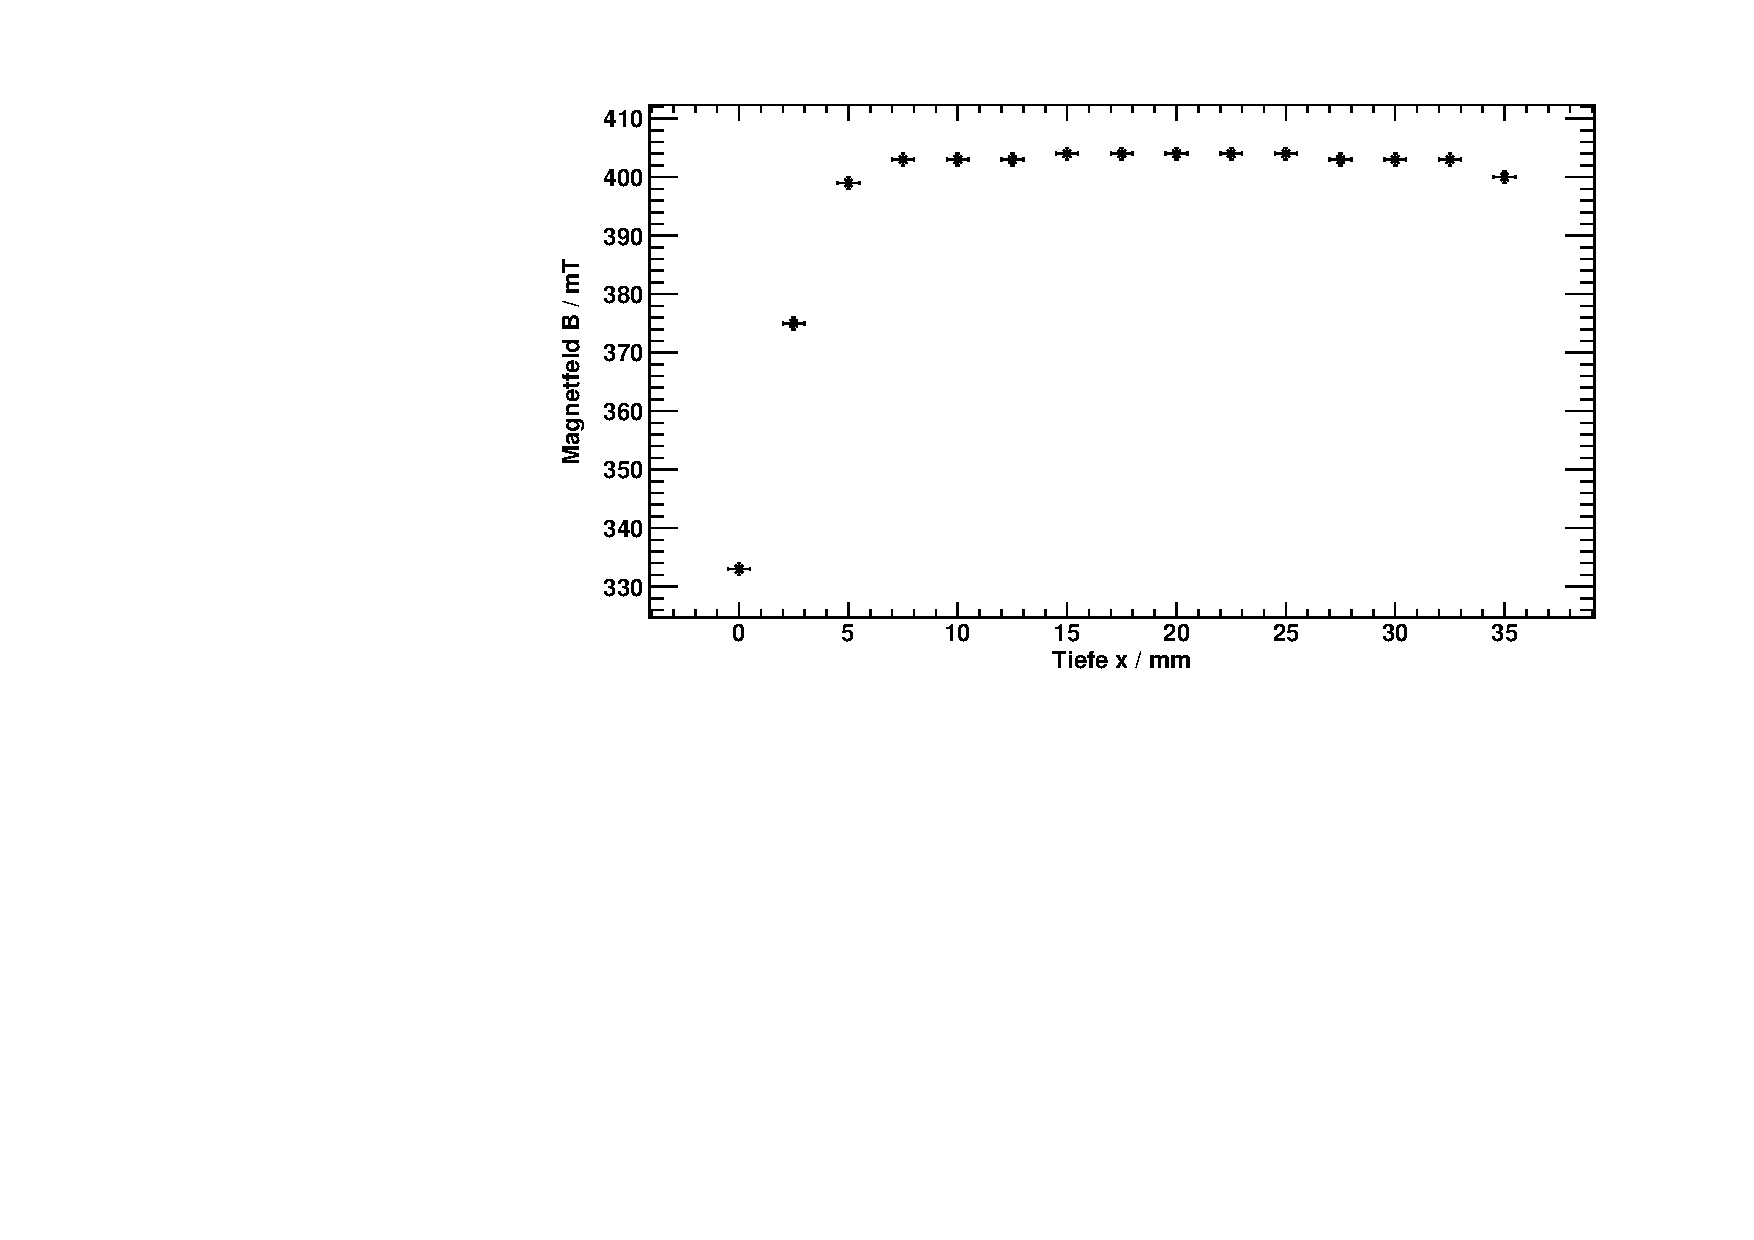
\includegraphics[width=\textwidth]{../img/01-B-x.pdf}
  \caption{Magnetfeldstärke $B$ in Abhängigkeit der Eindringtiefe $x$.}
  \label{img:B:x}
\end{center}
\end{figure}
\begin{figure}[H]
\begin{center}
  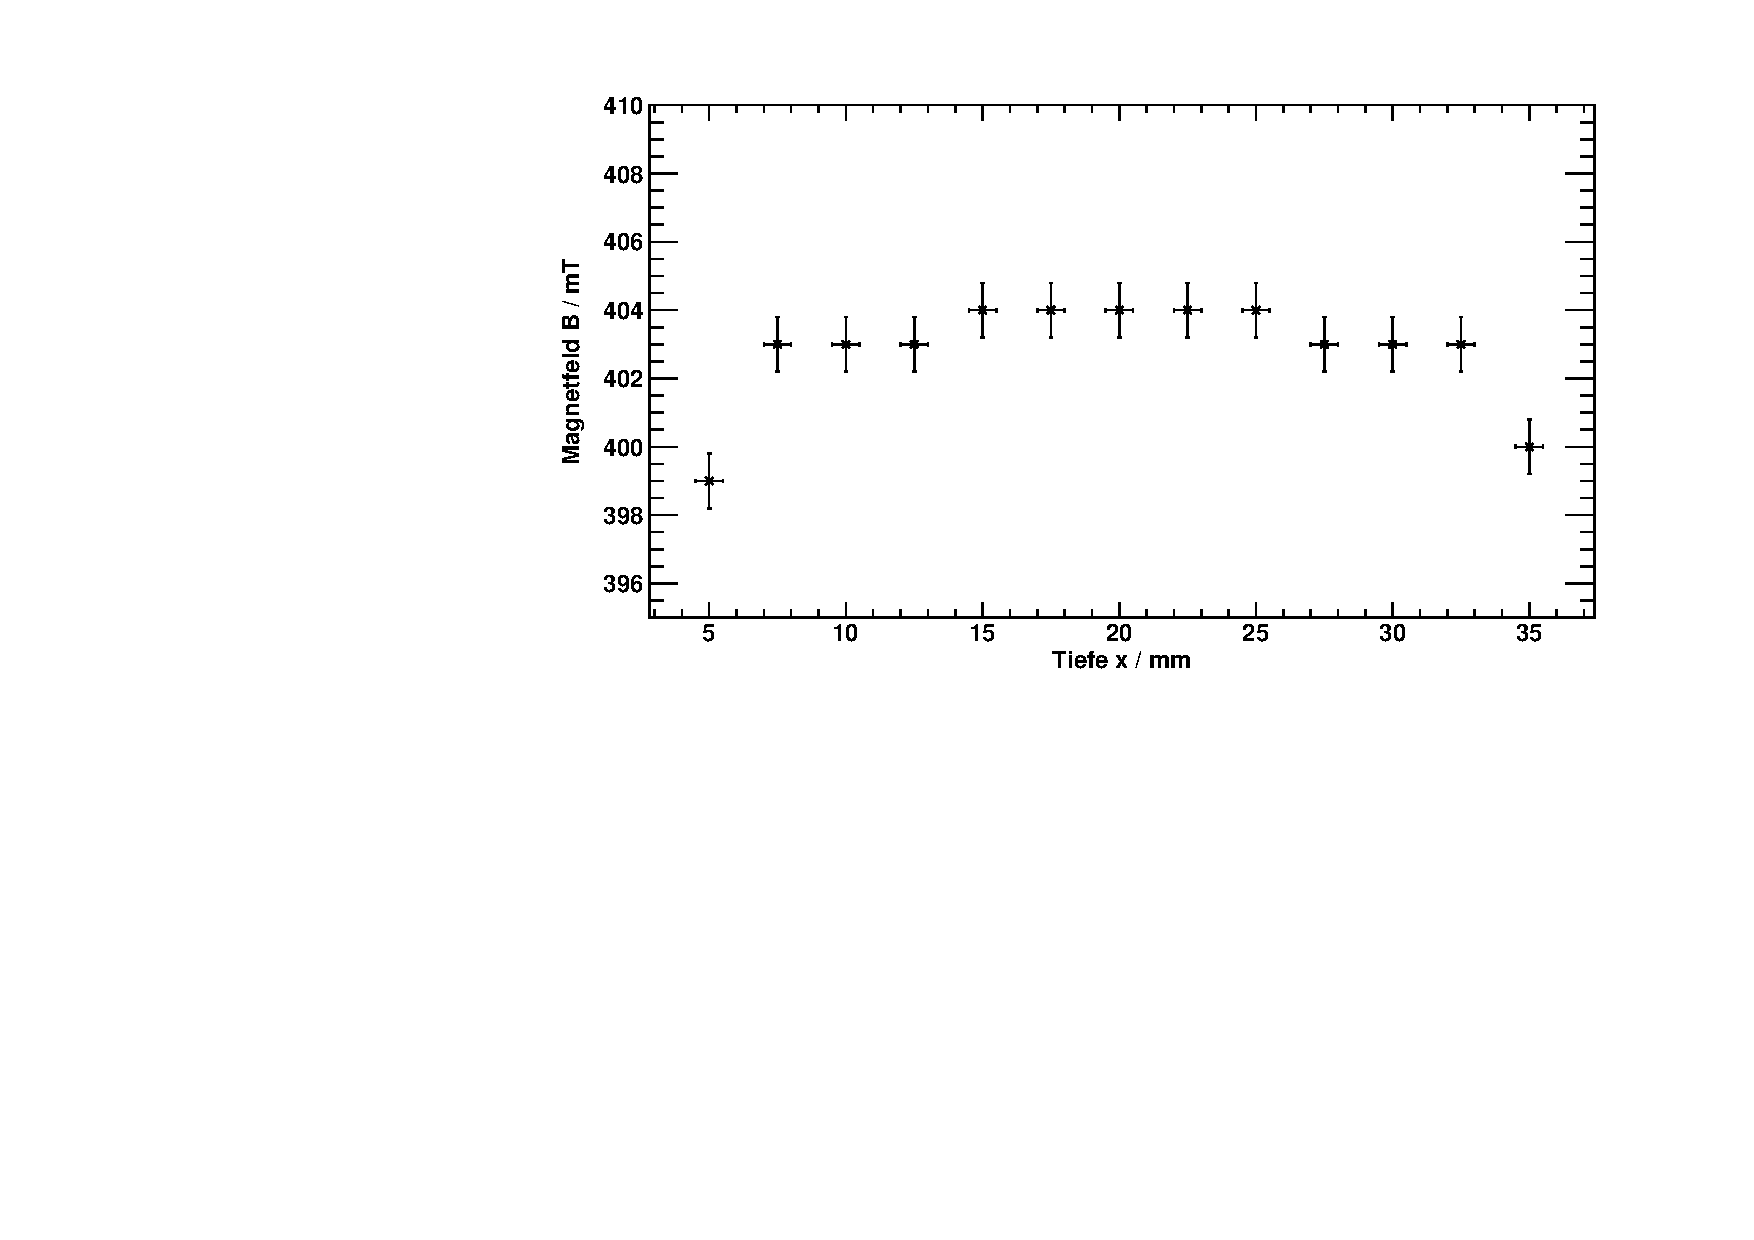
\includegraphics[width=\textwidth]{../img/01-B-x-zoom.pdf}
  \caption{Vergrößerung von \autoref{img:B:x}}
  \label{img:B:x:zoom}
\end{center}
\end{figure}

\subsubsection{Stromabhängigkeit}
\begin{figure}[H]
\begin{center}
  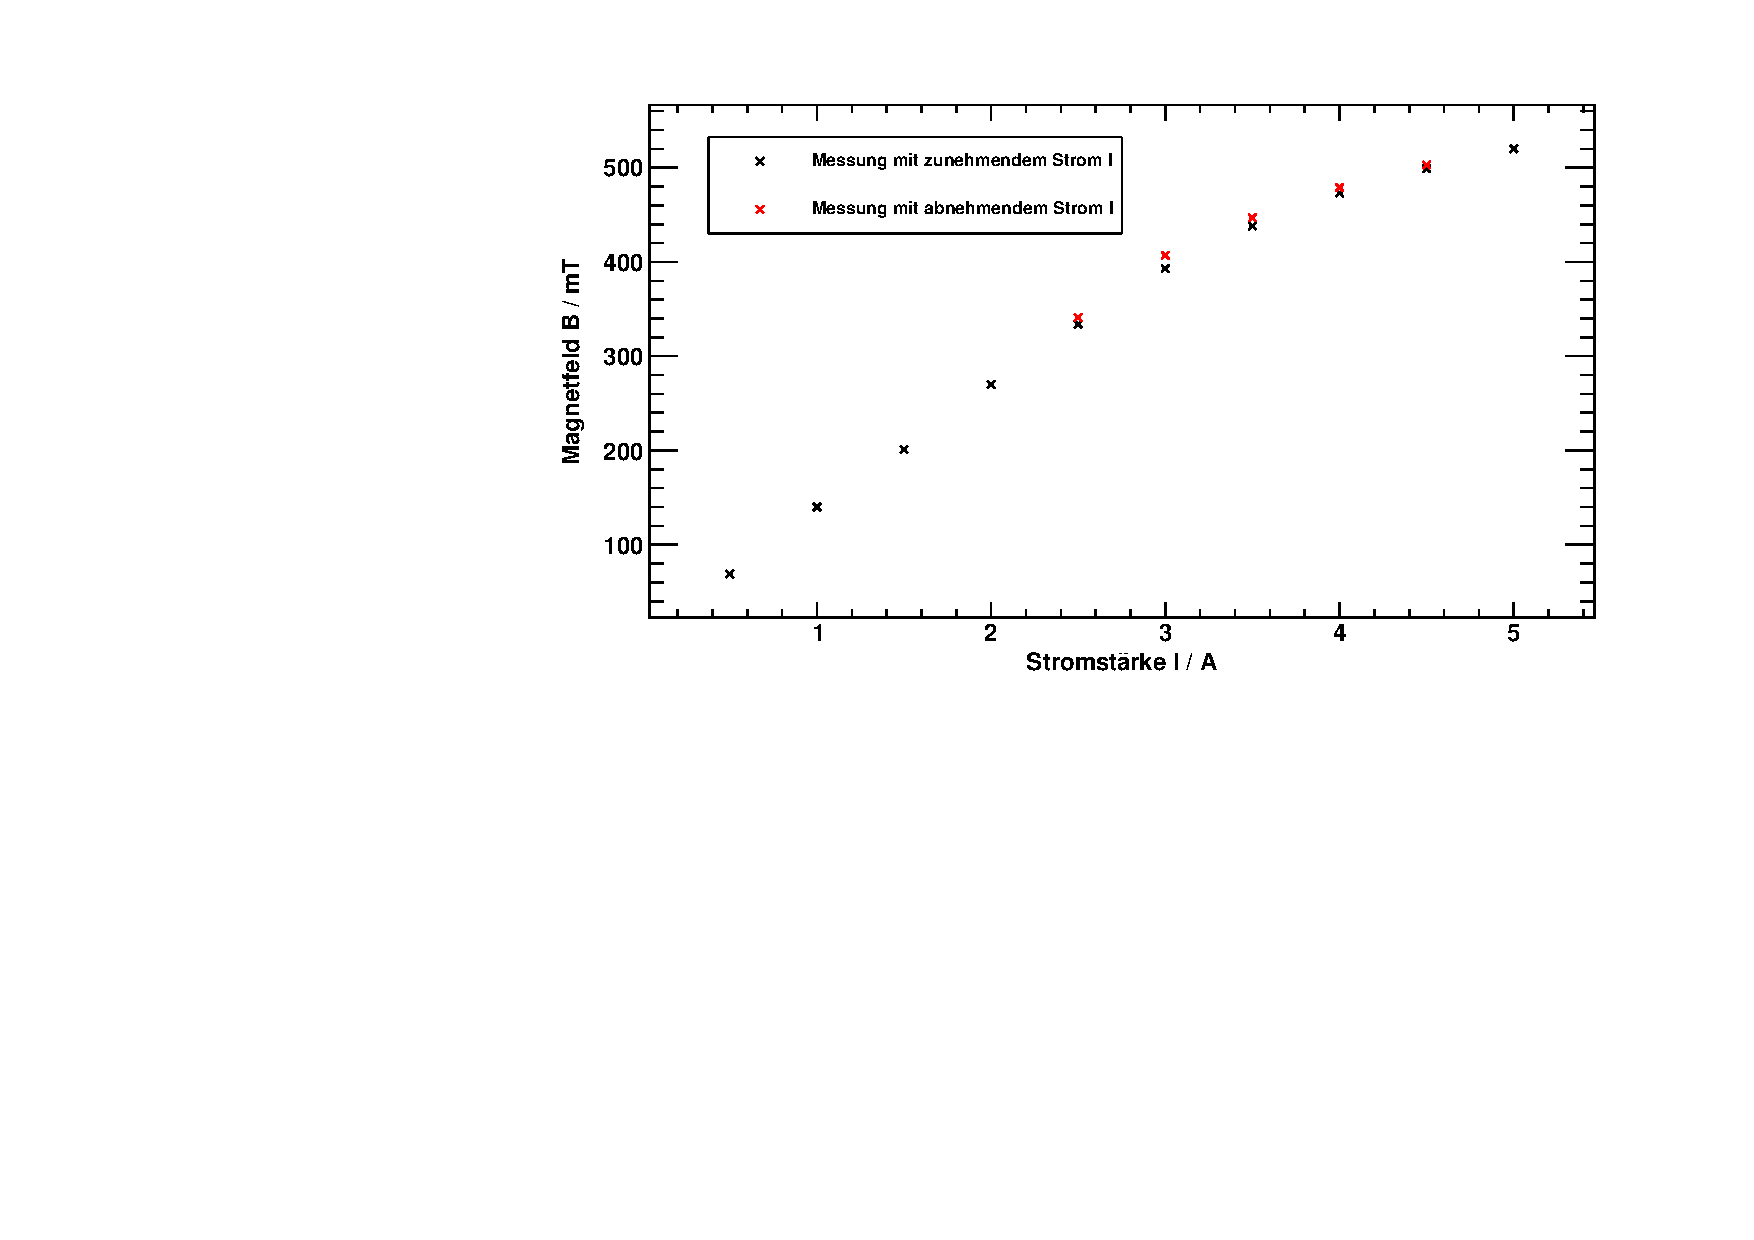
\includegraphics[width=\textwidth]{../img/02-B-I.pdf}
  \caption{Magnetfeldstärke $B$ in Abhängigkeit des Stroms $I$ und Richtung der Veränderung dessen.}
  \label{img:B:I}
\end{center}
\end{figure}
Hysterese

\subsection{Bestimmung der gyromagnetischen Verhältnisse}
\subsubsection{Bestimmung des Fehlers und Berechnung von $\gamma_H$}  %Fehler von B oder \gamma ?
\begin{figure}[H]
\begin{center}
  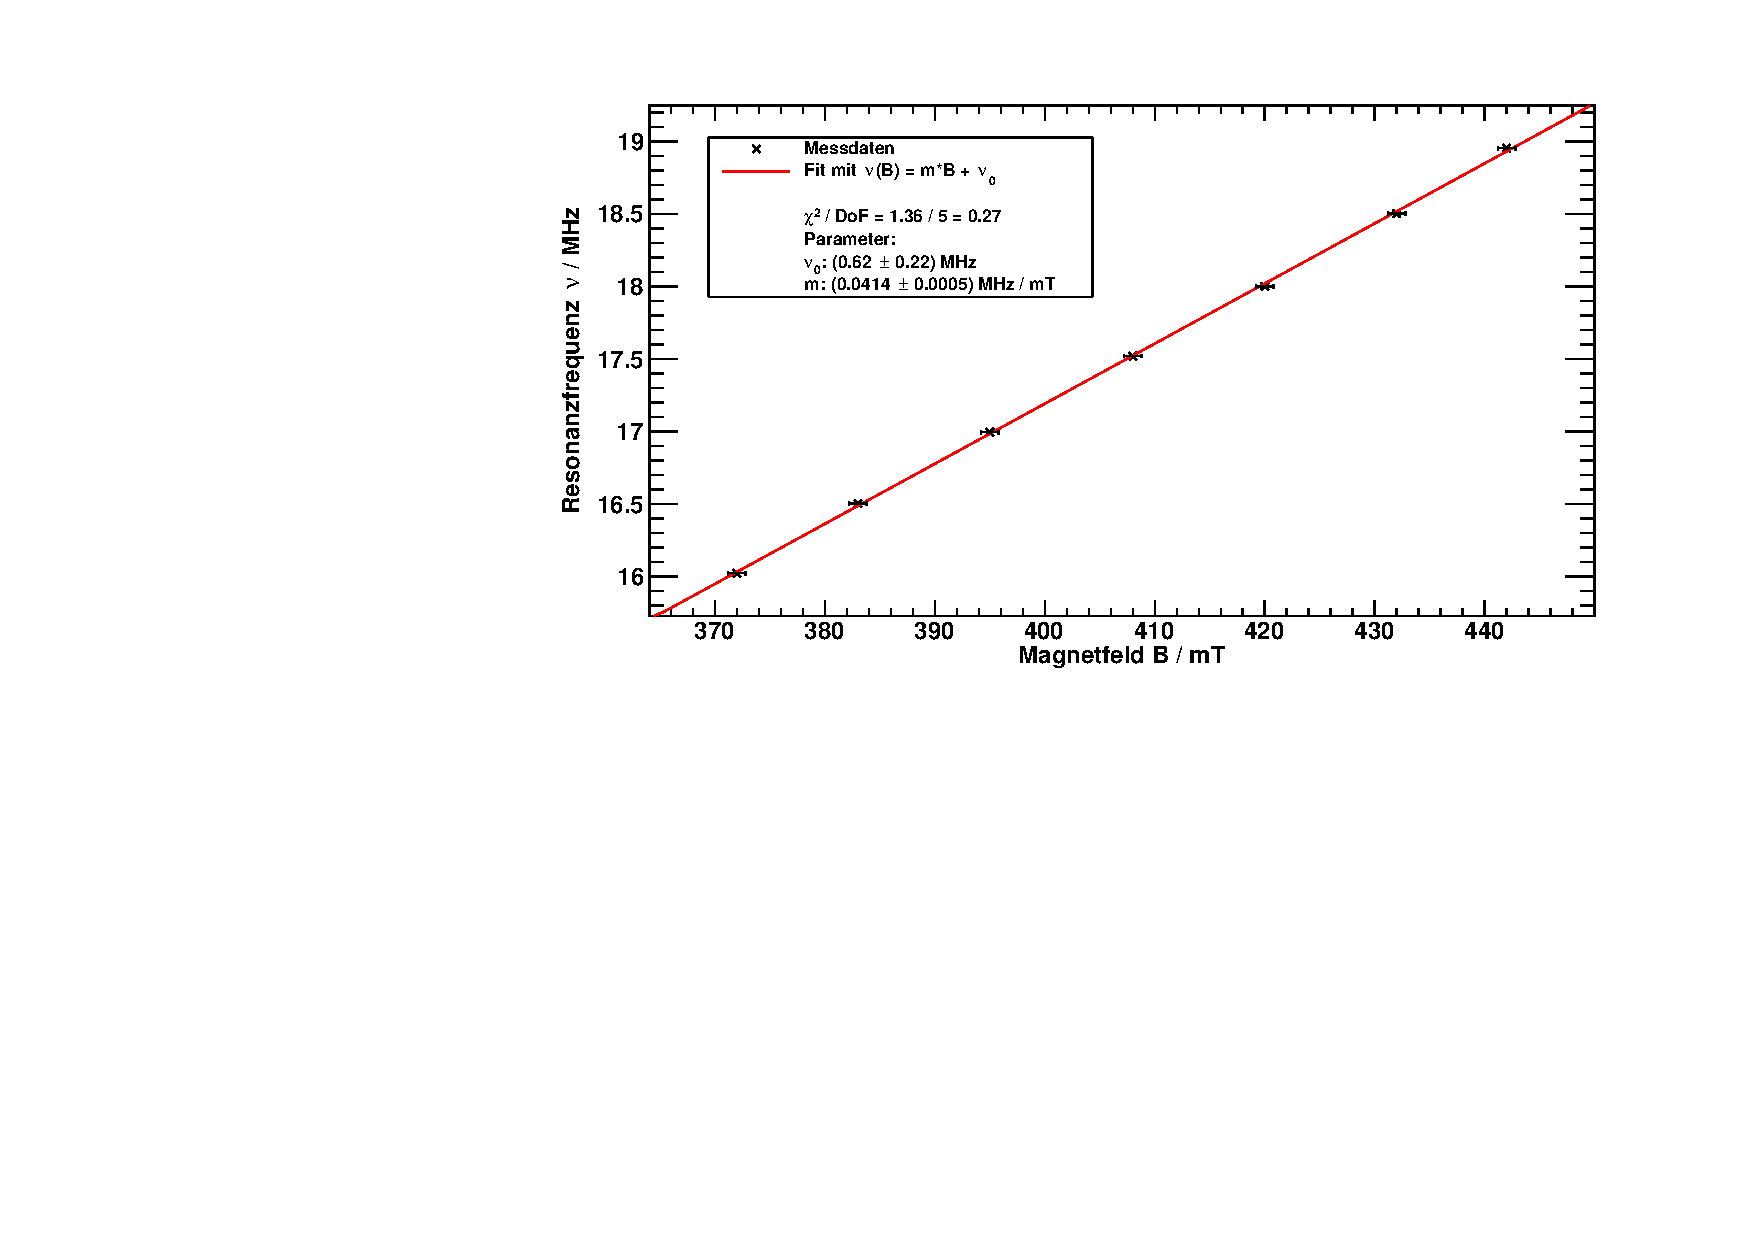
\includegraphics[width=\textwidth]{../img/03-H.pdf}
  \caption{Messungen der Resonanzfrequenzen $\nu$ für verschiedene Magnetfelder $B$.}
  \label{img:H}
\end{center}
\end{figure}

\subsubsection{Berechnung von $\gamma_\text{Glycol}$ und $\gamma_\text{Teflon}$}